\documentclass[conference]{IEEEtran}
\usepackage{cite}
\usepackage{url}
\usepackage{graphicx}
\usepackage{enumitem}
\usepackage{parskip}

\title{\vspace{-0.5cm}A Research Proposal for \\``Phylogenetic Analysis of lncRNAs Implicated in Alzheimer's Disease''}

\author{Derek Robinson, Mina Emadi, Mazyar Ghezelji\\
University of Victoria\\
Victoria, Canada \\
\{drobinson, minaemadi, mazyarghezelji\}@uvic.ca}

\begin{document}
\newlist{questions}{enumerate}{2}
\setlist[questions,1]{label=RQ\arabic*.,ref=RQ\arabic*}
\setlist[questions,2]{label=(\alph*),ref=\thequestionsi(\alph*)}

\maketitle

\section{Introduction}\label{sec:intro}

There is no doubt that Alzheimer's disease (AD) greatly affects the lives of those diagnosed and those who care for the diagnosed. 
In the United States, AD is currently the sixth leading cause of death for American adults \cite{AlzheimersDisease}. 
In Canada, over 747,000 patients are living with AD, or another form of dementia \cite{ADcanada}. 
While many humans suffer from AD, it is not well understood if other great apes (Hominidae) also suffer from AD. 
Finch and Austad argue that with our current understanding of AD, it is not possible to determine if AD is uniquely human \cite{finch2015commentary}.
As a group, we are interested in learning more about AD; specifically, the phylogeny of the long non-coding RNAs (lncRNAs) which have been implicated in AD \cite{luo2016long}. 
We have chosen to work on lncRNA as a majority of the human genome is transcribed into non-coding RNA sequences.

Our main objective for this research project is to build the phylogenetic tree for one of the lncRNAs implicated in AD, as identified by Luo and Chen \cite{luo2016long}. 
Our current target is brain cytoplasmic 200 (BC200) as we have already performed a preliminary BLAST search identifying several similar sequences to BC200 \cite{madden2012blast,blastTool}. 
Our secondary goal for this research project is to compare the structure of our lncRNA's most closely related homologs to shine light on the possible differences that may lead to AD being uniquely human.

Thus, our research questions are as follows:

\begin{questions}
    \item What does the phylogenetic tree of BC200 look like?
    \item What structural differences exist between BC200 and its two most closely related homologs?
\end{questions}

\section{Background}\label{sec:background}

\subsection{What is BC200?}

Brain Cytoplasmic 200 lncRNA RNA (BC200) is a 200 nucleotide long RNA transcript which is found mostly in the brain \cite{tiedge1993primary}. 
As a Non-coding RNA, BC200 is not translated into protein but can be used as a potential therapeutic target and biomarker due to its regulatory role in biological processes involved in disease development \cite{zhang2021role,mus2007dendritic}. 
This lncRNA has recently been studied extensively because of its role in regulating translation and inhibiting its initiation, as well as its impacts in pathogenesis of Alzheimer's disease and cancer \cite{zhang2021role,tiedge1993primary}. 
These non-coding RNAs are involved in translation control, thus they impact the synthesis of dendritic proteins which facilitates long-term plastic changes at the synapse \cite{mus2007dendritic}.

\subsection{The Relation Between AD and BC200}

Alzheimer's disease (AD) is a Neurodegenerative disease resulting from synaptic plasticity failure in neurons \cite{mus2007dendritic}. 
It is a complex disease, meaning that it involves multiple cell types and signaling pathways \cite{zhang2021role}.

AD occurs due to the accumulation of two proteins in the brain. 
One of them is beta-amyloid (A$\beta$) which accumulates in neurons, forms plaques, and disrupts cell functions. 
The other one is hyper-phosphorylated tau protein which in abnormal levels can form neurofibrillary tangles in neurons and block synaptic transmissions \cite{zhang2021role}.

A$\beta$, a cleavage product of the amyloid precursor protein (APP), is generated by b-site APP-cleaving enzyme1 (BACE1) and $\gamma$-secretase complex, and it strongly influences the pathogenesis of AD. 
Inhibition of BACE1 activity and the subsequent reduction in A$\beta$ levels may cure or prevent AD\cite{li2018identification,zhang2021role}.

BC200 facilitates AD pathogenesis by up-regulating A$\beta$ production through the modulation of BACE1 expression. 
The inhibition of BC200 significantly suppresses BACE1 expression, increases cell viability and reduces cell apoptosis in an AD model, and these effects are reversed by BC200 over-expression \cite{li2018identification,zhang2021role}.

Many researches have demonstrated the important role of BC200 in AD. 
El Mus \emph{et al.} \cite{mus2007dendritic} show that there are steady decline in BC200 level from age 49 to 86, but, in AD brain its level was substantially higher. 
They also observe that BC200 expression is increased in brain areas that are involved in AD and it is parallel with severity of disease. 
Huanyen Li \emph{et al.} \cite{li2018identification} establish an AD cell model overexpressing A$\beta$1- 42 to observe the effects of BC200 on the cell viability and apoptosis and to investigate the associated underlying mechanisms. 
They observe that BC200 and BACE1 were increased upon treatment with A$\beta$1-42, and inhibition of BC200 rescued this A$\beta$1-42-mediated dysfunction, as indicated by the interaction of BC200 directly targeting BACE1. 
Moreover, inhibition of BC200 increased AD cell growth and reduced cells apoptosis. 
They demonstrate that BC200 is a potent positive regulator of BACE1 in AD cells and in conclusion, lncRNA BC200 facilitates AD pathogenesis by up-regulating Aβ through BACE1.  					 			 		 	 

\section{Materials and Methods}\label{sec:methods}

The methods we will be applying are those similar to Amirmahani and Goharrizi \cite{amirmahani2018phylogenetic}. 
Specifically, we will be using the bioinformatics program NCBI-BLAST in order to identify homologs of our chosen lncRNA \cite{madden2012blast,blastTool}. 
Once we have identified several homologs of our chosen lncRNA, we will then perform the phylogenetic analysis using MEGA11 \cite{tamura2021mega11}. 
Our phylogenetic tree will be created via all available tree construction algorithms (Maximum Likelihood, Neighbour Joining, and Minimum-Evolution), and each of the results will be compared. 
Once we have built the phylogenetic tree, we will then compare the secondary structure of the three most closely related homologs using RNAz 2.0 \cite{gruber2010rnaz}.

\section{Results}\label{sec:results}

\subsection{Phylogenetic Tree of BC200}
TODO

\subsection{Structural difference between BC200 and its homologs}

Brain cytoplasmic 200 long non-coding RNA (or BC200 lncRNA) is a 200 nucleotide RNA transcript that is found predominantly in the brain. It's primary function is regulating translation by inhibiting its initiation.
It's role in AD is not fully understood, but research shows that Long noncoding RNA BC200 facilitates AD pathogenesis by upregulating AB through BACE1.\cite{li2018identification}
The BC200 structure consist of three main parts: A-rich domain, Alu domain and unique domain \cite{jung2014rna}.
\begin{figure}
  \centering
  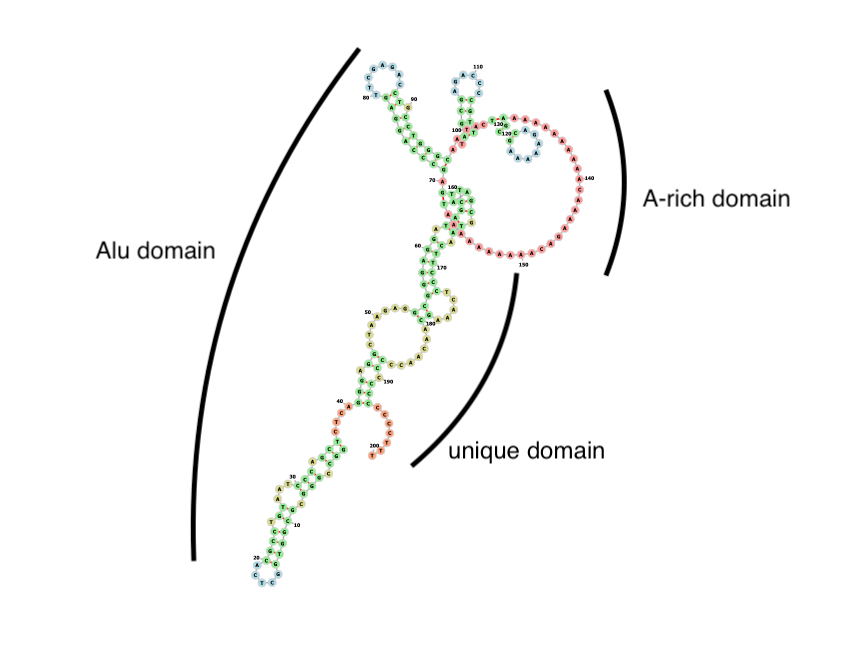
\includegraphics[width=0.4\textwidth]{figs/rna-6.png}
  \caption{BC200 RNA Secondary Structure}
\end{figure}
As we can see from the RNA secondary structures, all of the homologs have a nearly simialr A-rich domain, but on the other hand the the Alu domain is different between the homologs and BC200. The Alu domain of the mammalian signal recognition particle (SRP) comprises the heterodimer of proteins SRP9 and SRP14 bound to the 5′ and 3′ terminal sequences of SRP RNA\cite{weichenrieder2000structure}. So, their function in brain should be very different with eachother, eventhough there may be high similarity between their sequences.

\begin{figure}
  \centering
  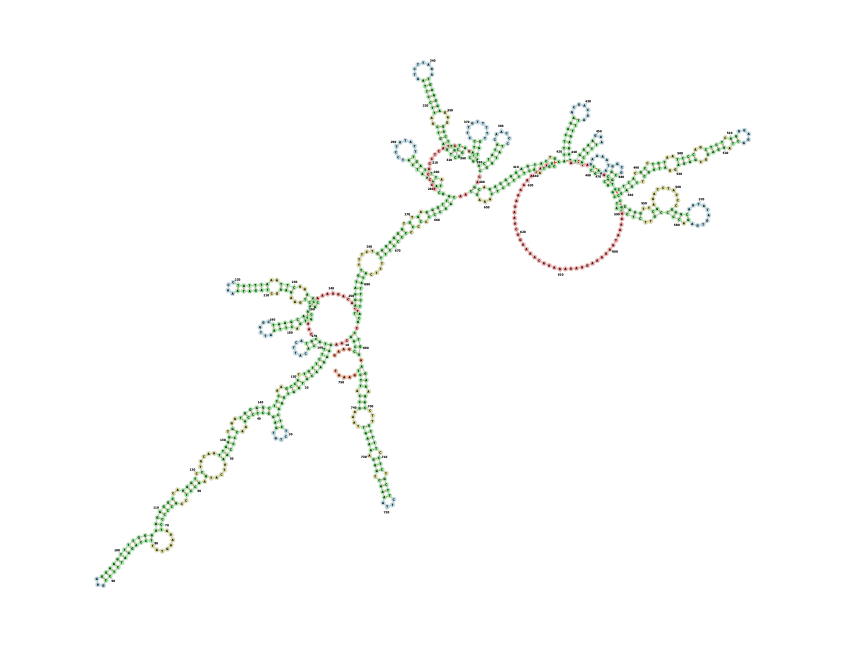
\includegraphics[width=0.4\textwidth]{figs/rnagorilla.png}
  \caption{BC200 RNA Secondary Structure in Gorilla}
\end{figure}
\begin{figure}
  \centering
  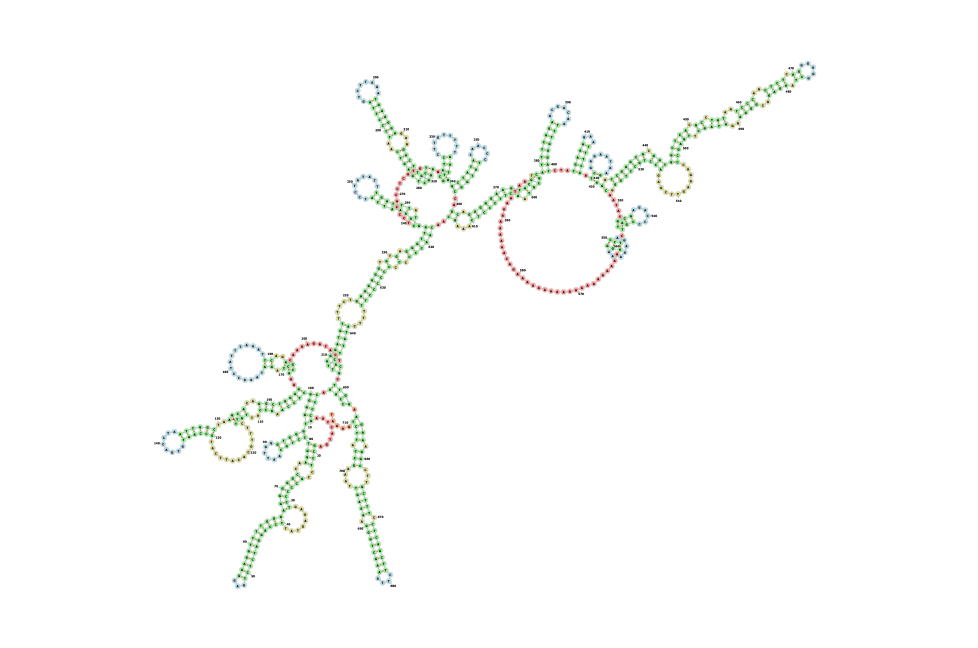
\includegraphics[width=0.4\textwidth]{figs/rnapan.png}
  \caption{BC200 RNA Secondary Structure in Pan}
\end{figure}
\begin{figure}
  \centering
  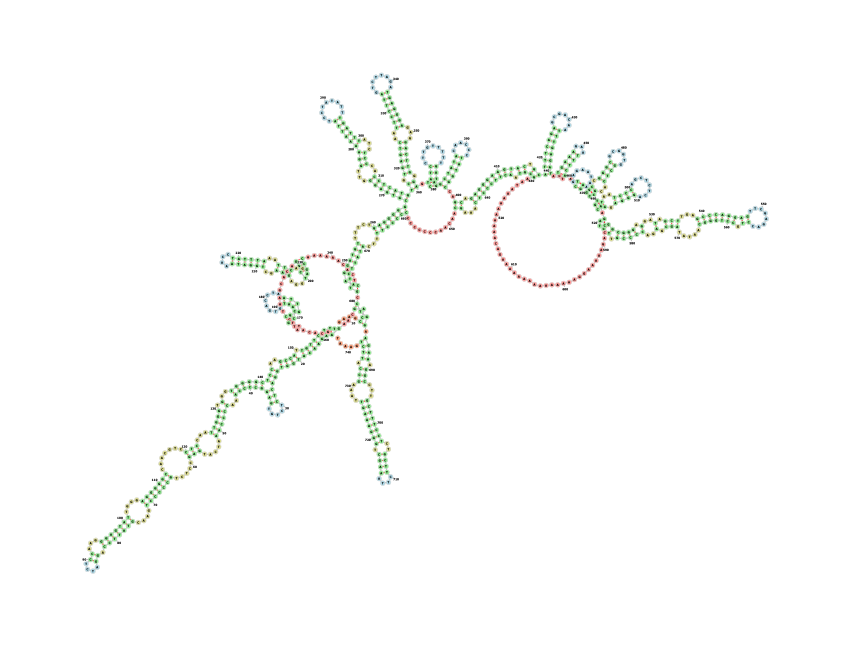
\includegraphics[width=0.4\textwidth]{figs/rnapango.png}
  \caption{BC200 RNA Secondary Structure in Pango}
\end{figure}

\subsection{Comparing BC200 sequence with its homologs}

One of the best ways for finding the conserved portions of a gene during evolution, is sequence alignment. Here, we aligned BC200 and the three most related homologs with each other to find the conserved parts of the sequence.

Here are the alignment results:
\begin{figure}
  \centering
  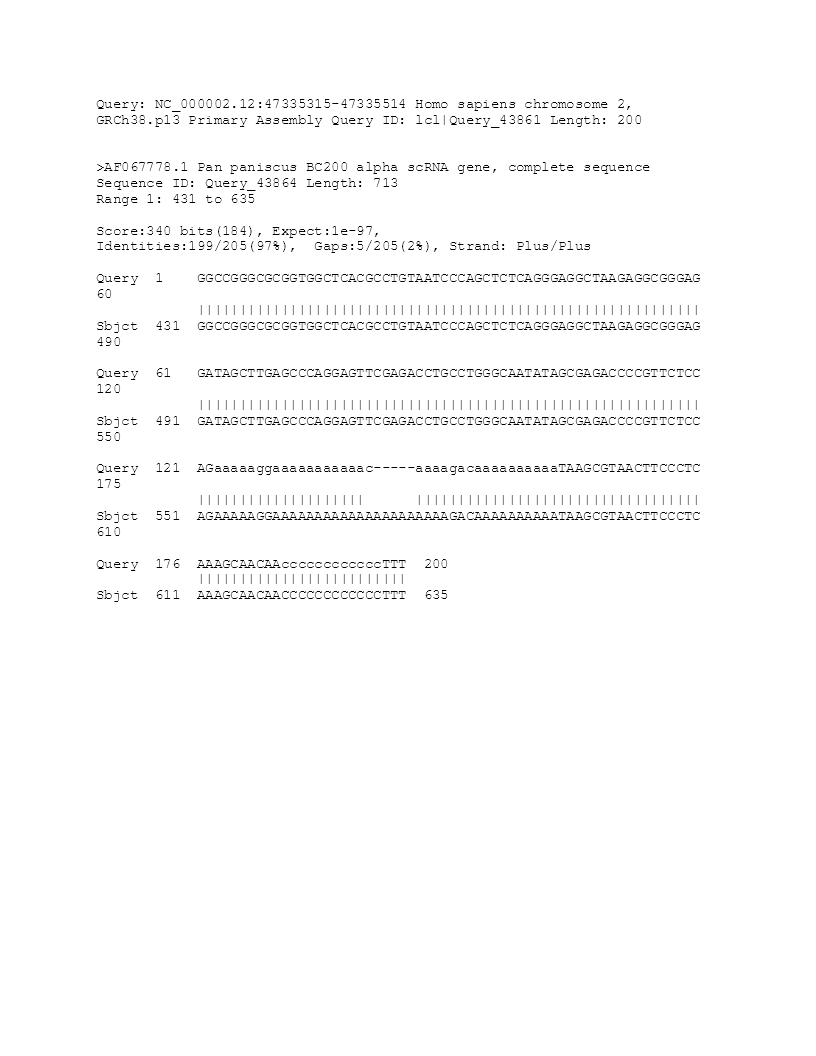
\includegraphics[width=0.4\textwidth]{figs/TK1PBYHT114-Alignment-2-page-1.png}
  \caption{BC200 Sequence Alignment with BC200 in pan}
\end{figure}
\begin{figure}
  \centering
  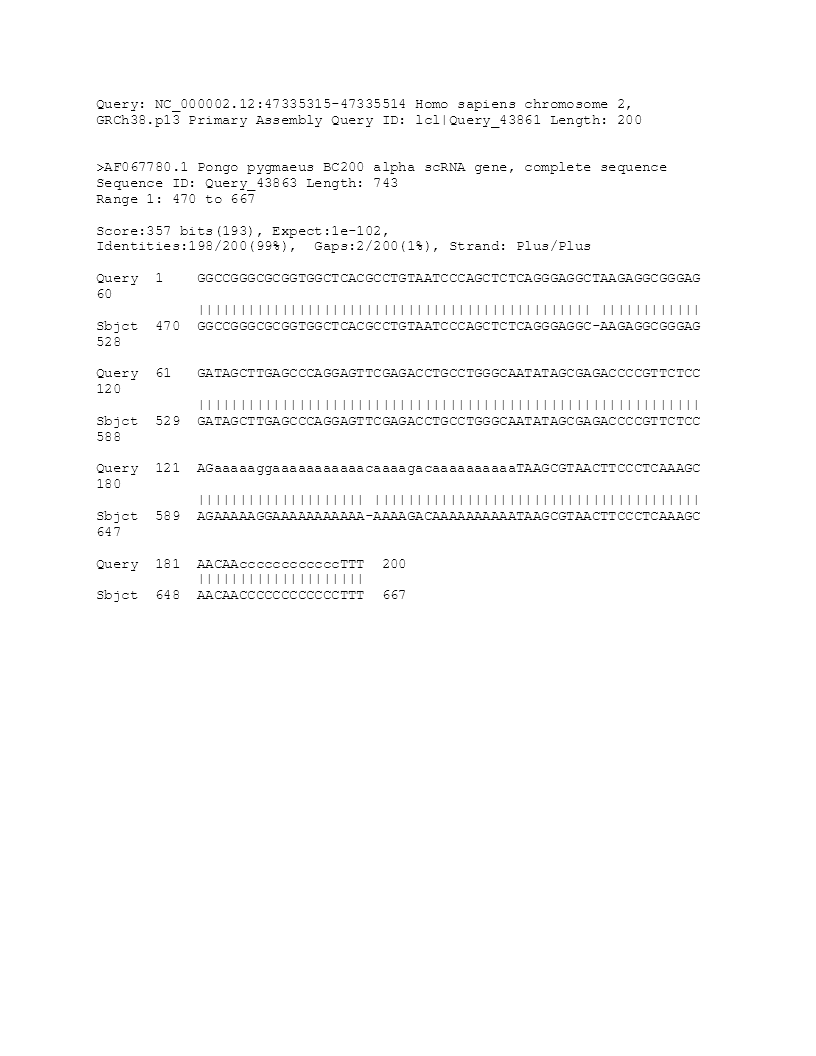
\includegraphics[width=0.4\textwidth]{figs/TK1PBYHT114-Alignment-3-page-1.png}
  \caption{BC200 Sequence Alignment with BC200 in Pango}
\end{figure}
\begin{figure}
  \centering
  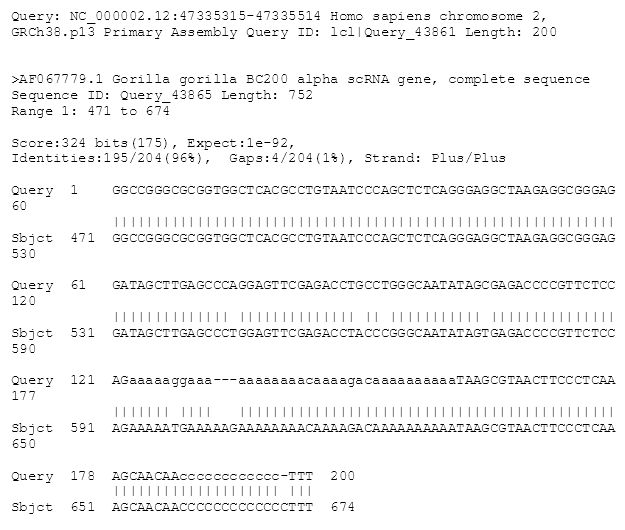
\includegraphics[width=0.4\textwidth]{figs/TK1PBYHT114-Alignment-page-1.png}
  \caption{BC200 Sequence Alignment with BC200 in Gorilla}
\end{figure}

As it is obvious from the results, most parts of the sequence are conserved. Which shows that there should be a high similarity between BC200 RNA in human body and in other species. So, the following result does not support our hypothesis, and they suggest that Alzheimer’s can be shared between human and great apes.

\section{Discussion}\label{sec:discussion}
TODO

\section{Conclusion}\label{sec:conclusion}
TODO

\bibliographystyle{IEEEtran}
\bibliography{refs.bib}
\end{document}